\subsection{Lệnh xargs}
\underline{\textbf{Chức năng của lệnh:}} Lệnh \verb|xargs <cmd> [args]| được dùng để thực thi lệnh được nhập từ đầu vào tiêu chuẩn bằng cách chuyển các chuỗi ký tự đầu vào thành lệnh và các đối số tương ứng \cite{mit-xv6} \cite{xargs}.

\underline{\textbf{Thiết lập thuật toán:}} (có tham khảo qua source code ở \cite{xargscode})

Hàm \mintinline{C++}|void clear(char** x_argv, int start)| được thiết lập để xóa câu lệnh đã được thực thi trước đó (vị trí bắt đầu từ \verb|start|).
Hàm \verb|main|:
\begin{enumerate}[labelindent=1em, labelsep=0.2cm, leftmargin=1cm, wide=\parindent, topsep=0.1cm, itemsep=-1ex, partopsep=1.5ex, parsep=1.5ex]
	\item Kiểm tra cú pháp của \verb|xargs|. Lệnh sẽ báo lỗi khi người dùng nhập sai cú pháp hoặc quá nhiều cú pháp (\verb|argc| vượt quá \verb|MAXARG|).
	\item Khởi tạo chuỗi \verb|buffer| để lưu các ký tự đầu, mảng các chuỗi \verb|x_argv| để lưu các chuỗi liền mạch trong \verb|buffer| và \verb|x_argc| để lưu số lượng chuỗi trong \verb|x_argv|.
	\item Đọc các ký tự sử dụng vòng lặp \verb|while|.
	\item Phân chia tiến trình bằng hàm \verb|fork()|. Tiến trình con sẽ đảm nhiệm việc chạy chương trình lưu trong \verb|x_argv|, trong khi tiến trình cha giải phóng vùng nhớ của các chuỗi trong câu lệnh đã được thực hiện trước đó. Chương trình kết thúc khi không còn ký tự đầu vào nào nữa.
\end{enumerate}

\underline{\textbf{Khó khăn đã gặp phải:}}
\begin{itemize}[labelindent=1em, labelsep=0.2cm, leftmargin=1cm, wide=\parindent, topsep=0.1cm, itemsep=-1ex, partopsep=1.5ex, parsep=1.5ex]
	\item Hiểu đúng nguyên lý hoạt động của \verb|xargs| trên Unix.
	\item Việc đọc và lưu trữ ký tự phải được thực hiện kỹ càng để không bỏ sót các lệnh/đối số hoặc đọc sai lệnh/đối số.
\end{itemize}

Dưới đây là kết quả chạy thử trên \verb|qemu| và kiểm tra lệnh \verb|xargs| bằng chương trình kiểm thử:
\begin{figure}[htp!]
	\centering
	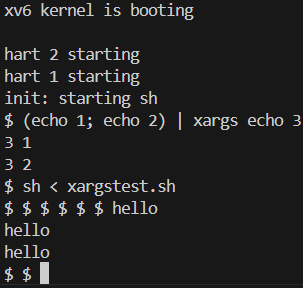
\includegraphics[width=0.5\textwidth]{figures/exec-xargs}
	\caption{Kết quả chạy thử \textbf{xargs} trên \textbf{qemu}}
\end{figure}
\begin{figure}[htp!]
	\centering
	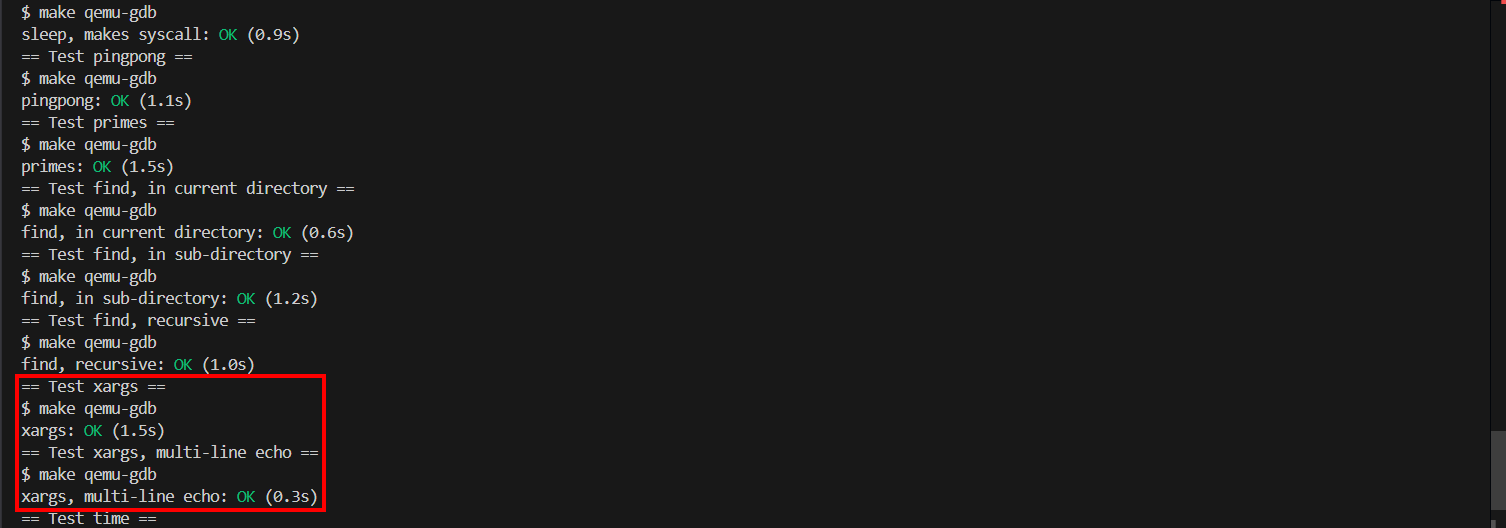
\includegraphics[width=0.9\textwidth]{figures/xargs-test}
	\caption{Kết quả kiểm thử \textbf{xargs} bằng công cụ chấm bài \textbf{grade} của MIT}
\end{figure}